\section{Results}
    Will contain a presentation of the various spectral fitting results in figures and tables.

    To perform fitting of NICER data \cite{orio2022nicer}

    \subsection{Observed count rates}
    In figure \ref{fig:all-counts}, we present a comparison of count rates derived from the multiple observations listed in table ***. Figure \ref{fig:all-counts:unnorm} is constructed to illustrate the variability of flux across different observation epochs, with count rates plotted on a logarithmic scale. This visualization provides insights into the temporal evolution of X-ray emission from MR Vel.

    \begin{figure*}[!htb]
        \centering
        \begin{subfigure}[b]{0.45\textwidth}
            \centering
            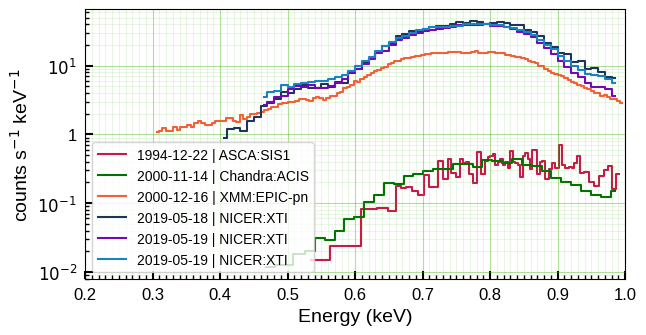
\includegraphics[width=\textwidth]{figures/ldata/mr-vel-counts_all-obs.png}
            \caption{Comparison of flux from all observations from their count rates plotted to scale}
            \label{fig:all-counts:unnorm}
        \end{subfigure}
        \hfill
        \begin{subfigure}[b]{0.45\textwidth}
            \centering
            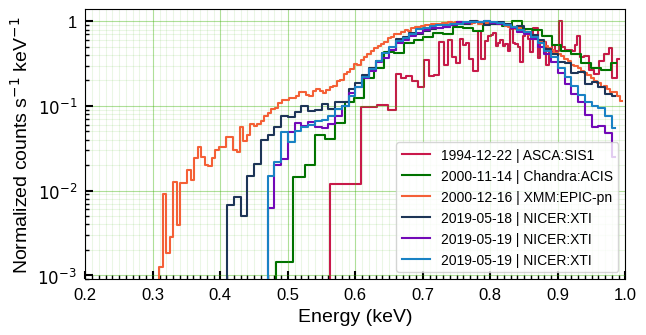
\includegraphics[width=\textwidth]{figures/ldata/mr-vel-normcounts_all-obs.png}
            \caption{Normalized count rates from all observations show varying responses to supersoft X-rays}
            \label{fig:all-counts:norm}
        \end{subfigure}
        \caption{Count rates from observational dataset}
        \label{fig:all-counts}
    \end{figure*}
    
    Concurrently, in figure \ref{fig:all-counts:norm}, the count rates are normalized to the range of 0 to 1 using \textit{min-max normalization}. This visualization accentuates the relative sensitivity of more recent observations to supersoft X-ray photons emitted by MR Vel. The sub-plot underscores the enhanced discernibility of X-ray features in recent observations, suggestive of improved observational capabilities or heightened sensitivity to the emitted X-ray flux.
    
    Together, these visualizations offer a nuanced understanding of the flux variability and observational sensitivity trends exhibited by MR Vel across different observation epochs, contributing to the broader understanding of its X-ray emission characteristics.

    \subsection{Unfolded spectra}
    % \begin{figure*}[!htb]
    %     \centering
    %     \begin{subfigure}[b]{0.45\textwidth}
    %         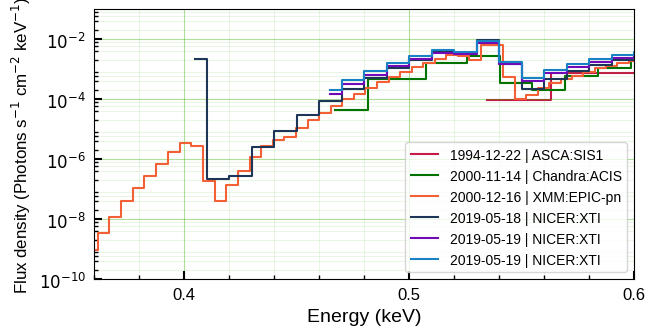
\includegraphics[width=\textwidth]{figures/eufspec/mr-vel-uf-keV_all-obs_360-600.png}
    %         \caption{Unfolded spectra after model fitting for the range 0.36 keV - 0.6 keV}
    %         \label{fig:all-uf-keV:360-600}
    %     \end{subfigure}
    %     \hfill
    %     \begin{subfigure}[b]{0.45\textwidth}
    %         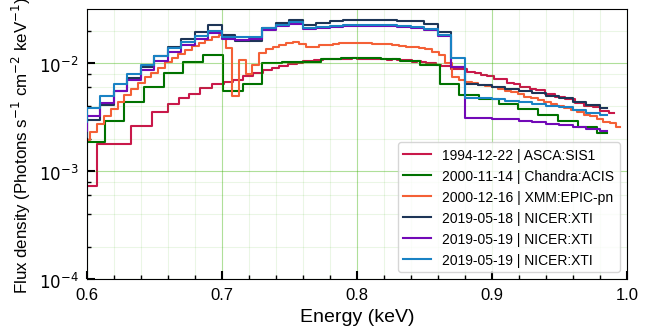
\includegraphics[width=\textwidth]{figures/eufspec/mr-vel-uf-keV_all-obs_600-1000.png}
    %         \caption{Unfolded spectra after model fitting for the range 0.6 keV - 1.0 keV}
    %         \label{fig:all-uf-keV:600-1000}
    %     \end{subfigure}
    %     \caption{Unfolded spectral after model fitting}
    %     \label{fig:all-uf-keV}
    % \end{figure*}
    \begin{figure*}[!htb]
        \centering
        \begin{subfigure}[b]{0.45\textwidth}
            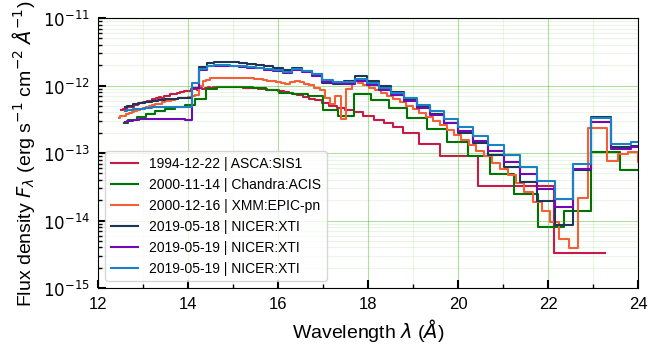
\includegraphics[width=\textwidth]{figures/eufspec/mr-vel-uf_all-obs_12-24.png}
            \caption{Unfolded spectra after model fitting in the range 12 \AA - 24 \AA}
            \label{fig:all-uf:12-24}
        \end{subfigure}
        \hfill
        \begin{subfigure}[b]{0.45\textwidth}
            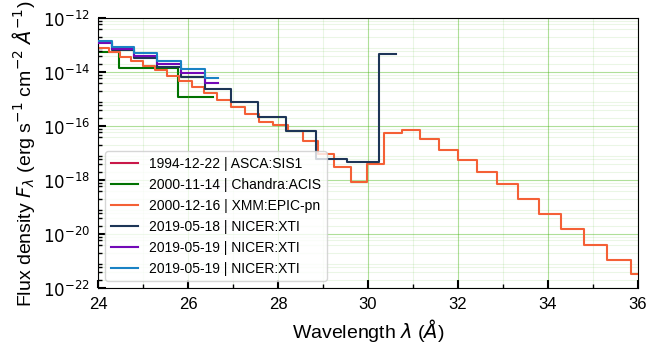
\includegraphics[width=\textwidth]{figures/eufspec/mr-vel-uf_all-obs_24-36.png}
            \caption{Unfolded spectra after model fitting in the range 24 \AA - 36 \AA}
            \label{fig:all-uf:24-36}
        \end{subfigure}
        \caption{Unfolded spectral after model fitting}
        \label{fig:all-uf}
    \end{figure*}
